\documentclass[conference]{IEEEtran}
\IEEEoverridecommandlockouts
\usepackage{cite}
\usepackage{amsmath,amssymb,amsfonts}
\usepackage{algorithmic}
\usepackage{graphicx}
\usepackage{textcomp}
\usepackage{xcolor}
\def\BibTeX{{\rm B\kern-.05em{\sc i\kern-.025em b}\kern-.08em
		T\kern-.1667em\lower.7ex\hbox{E}\kern-.125emX}}
\begin{document}
	
	\title{FPGA Implementation of FIR Filter Using Vivado FIR Compiler and DMA Interfacing on Zynq SoC}
	
	\author{\IEEEauthorblockN{Athi Ram S}
		\IEEEauthorblockA{\textit{Department of Electronics and Communication Engineering} \\
			\textit{R.M.K. Engineering College}\\
			Tamil Nadu, India \\
			athiramr.s@rmkec.ac.in}
	}
	
	\maketitle
	
	\begin{abstract}
		This paper presents the design and hardware implementation of a Finite Impulse Response (FIR) filter using the Vivado FIR Compiler IP on a Zynq SoC. The project demonstrates the interfacing between the Processing System (PS) and Programmable Logic (PL) using AXI DMA for real-time signal processing. Experimental results validate the correctness and efficiency of the design, achieving a hardware execution time of 0.005709 seconds compared to 0.055059 seconds in software, confirming the performance improvement through FPGA acceleration.
	\end{abstract}
	
	\begin{IEEEkeywords}
		FPGA, FIR Filter, Zynq SoC, Vivado HLS, DMA, Hardware Acceleration
	\end{IEEEkeywords}
	
	\section{Introduction}
	Finite Impulse Response (FIR) filters are essential components in digital signal processing applications such as communication systems, audio enhancement, and biomedical signal analysis. Implementing these filters on Field Programmable Gate Arrays (FPGAs) provides significant performance advantages due to parallelism and pipelining capabilities.
	
	In this work, we utilize the Xilinx Vivado FIR Compiler IP to design and implement an efficient FIR filter. The design is mapped onto a Zynq SoC platform (PYNQ-Z2), leveraging the ARM processing system (PS) and programmable logic (PL) for efficient hardware-software co-design.
	
	\section{Literature Review}
	
	\subsection{Improved Implementation of PYNQ-Based FFT Hardware Accelerator}
	\textbf{Authors:} Kartik Agrawal, Abhijit Asati \\
	\textbf{Published:} 2024 IEEE
	
	\noindent In recent times, the idea of hardware accelerators has gained considerable traction, particularly with the advent of Field Programmable Gate Arrays (FPGAs) that allow speeding up commonly used software functions. The interest further increased with Xilinx’s introduction of the Python Productivity for Zynq (PYNQ) framework, which simplifies the design and control of such accelerators. In this study, the authors designed a hardware accelerator for a Fast Fourier Transform (FFT) filter using PYNQ. Its performance was compared with the software implementation available in the NumPy library and with prior FFT accelerator designs that utilized custom Direct Memory Access (DMA) IPs. 
	Unlike complex custom IP designs requiring specialized architecture knowledge, this work employed standard Vivado DMA IP along with a fixed-size FFT configuration, achieving competitive or superior performance with reduced hardware utilization. The paper also proposed a technique to employ the fixed-size FFT for varying input sample sizes at runtime. Comparative analysis for delay, resource consumption, and power usage demonstrated significant efficiency, providing design insights for future FPGA-based accelerators.
	
	\subsection{Equiripple FIR Filter Design by the FFT Algorithm}
	\textbf{Authors:} A.E. Cetin, O.N. Gerek, Y. Yardimci \\
	\textbf{Published:} 2024 IEEE
	
	\noindent This paper presents a simple and effective procedure for designing finite-extent impulse response (FIR) filters using the Fast Fourier Transform (FFT) algorithm. The zero-phase (linear phase) FIR filter design problem is formulated to alternately satisfy both frequency-domain magnitude constraints and time-domain impulse support constraints. The proposed iterative approach performs two FFT computations per iteration to refine the filter response, yielding an equiripple approximation to the desired frequency characteristics. The FFT-based design’s major advantages are its simplicity, computational efficiency, and adaptability to higher-dimensional filter design, which is challenging for classical approaches such as the Parks–McClellan algorithm. The authors emphasize that while Parks–McClellan is highly efficient for one-dimensional cases, it cannot be easily generalized to multidimensional filters, whereas their FFT-based method can.
	
	\subsection{Implementation of FIR Digital Filter Algorithm in C Language on DSP Platform}
	\textbf{Author:} Guoyong Wang \\
	\textbf{Published:} 2024 IEEE
	
	\noindent This study details the implementation of a Finite Impulse Response (FIR) digital filter on a Texas Instruments TMS320-series DSP platform using the C programming language. The paper systematically covers the FIR filter’s working principles, design methodologies, DSP development environment, code implementation, simulation verification, and hardware testing. Through simulation, the frequency response characteristics were validated, and system-level testing confirmed accurate signal filtering performance, high signal-to-noise ratio, and low distortion. The research highlights that FIR filters implemented on dedicated DSP hardware deliver excellent signal processing performance, offering a practical framework for FIR-based real-time embedded systems.
	
	\subsection{Implementation of Distributed FIR Digital Filter on FPGA}
	\textbf{Authors:} Xiao Liangfen, Liu Yi \\
	\textbf{Published:} 2023 IEEE
	
	\noindent The rapid development of digital filtering techniques has enabled digital filters to replace analog counterparts in numerous applications. This paper presents a design methodology for a distributed FIR digital filter implemented on FPGA. The distributed arithmetic approach effectively reduces multiplication overhead, enabling efficient use of FPGA resources. The implementation process, simulation verification, and experimental results demonstrate the approach’s validity, showcasing low latency, compact hardware utilization, and stable frequency response. The study concludes that distributed FIR filters implemented on FPGA provide a flexible, high-performance alternative for real-time digital signal processing applications.
	
	\subsection{Summary of Literature Insights}
	From the reviewed literature, it is evident that FPGA-based implementations of DSP algorithms provide significant acceleration and flexibility over traditional DSP processors and software-only methods. The use of frameworks such as PYNQ simplifies integration, while FIR and FFT algorithm optimizations continue to evolve toward resource-efficient designs. Techniques like distributed arithmetic and FFT-based equiripple design offer reduced computational overhead and scalability. The reviewed studies collectively demonstrate that FPGA-based acceleration is becoming a mainstream method for implementing real-time signal processing applications, providing the foundation for this project’s FIR filter implementation on the Zynq SoC.
	
	\section{System Design}
	The FIR filter architecture is developed using the Vivado IP Integrator environment. Fig.~\ref{fig_block} shows the primary block diagram illustrating the interaction between the PS and PL through AXI DMA and the FIR Compiler IP.
	
	\begin{figure}[htbp]
		\centerline{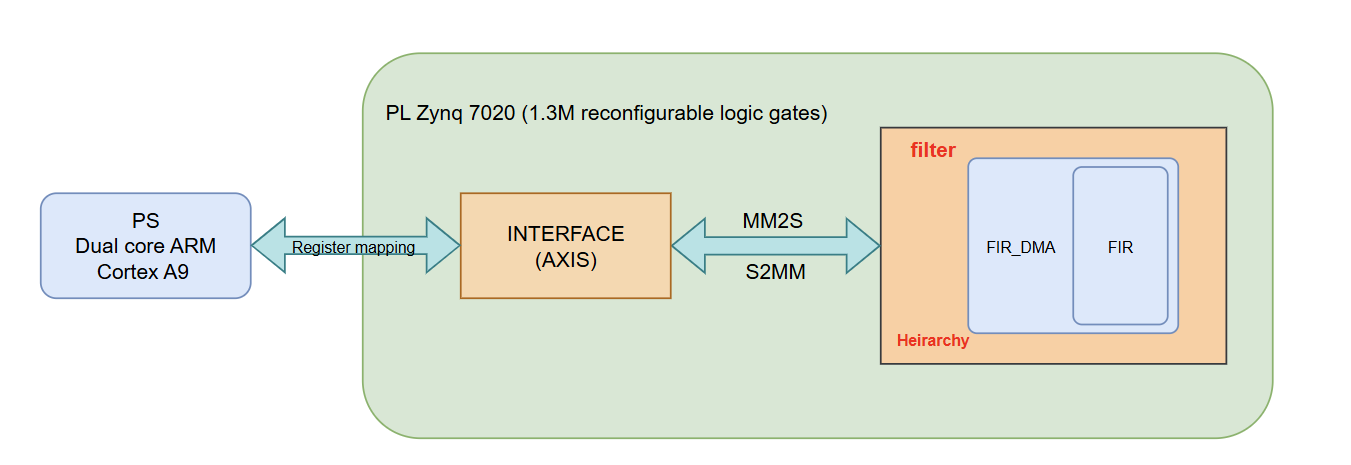
\includegraphics[width=0.47\textwidth]{blockdiagram.png}}
		\caption{Mapping of PS, PL, and FIR Compiler IP interfaces.}
		\label{fig_block}
	\end{figure}
	
	\subsection{Coefficient Configuration}
	The FIR coefficients and associated configurations were defined using the Vivado FIR Compiler GUI as shown in Fig.~\ref{fig_coeff}. The coefficients correspond to a low-pass filter design with quantized fixed-point representation.
	
	\begin{figure}[htbp]
		\centerline{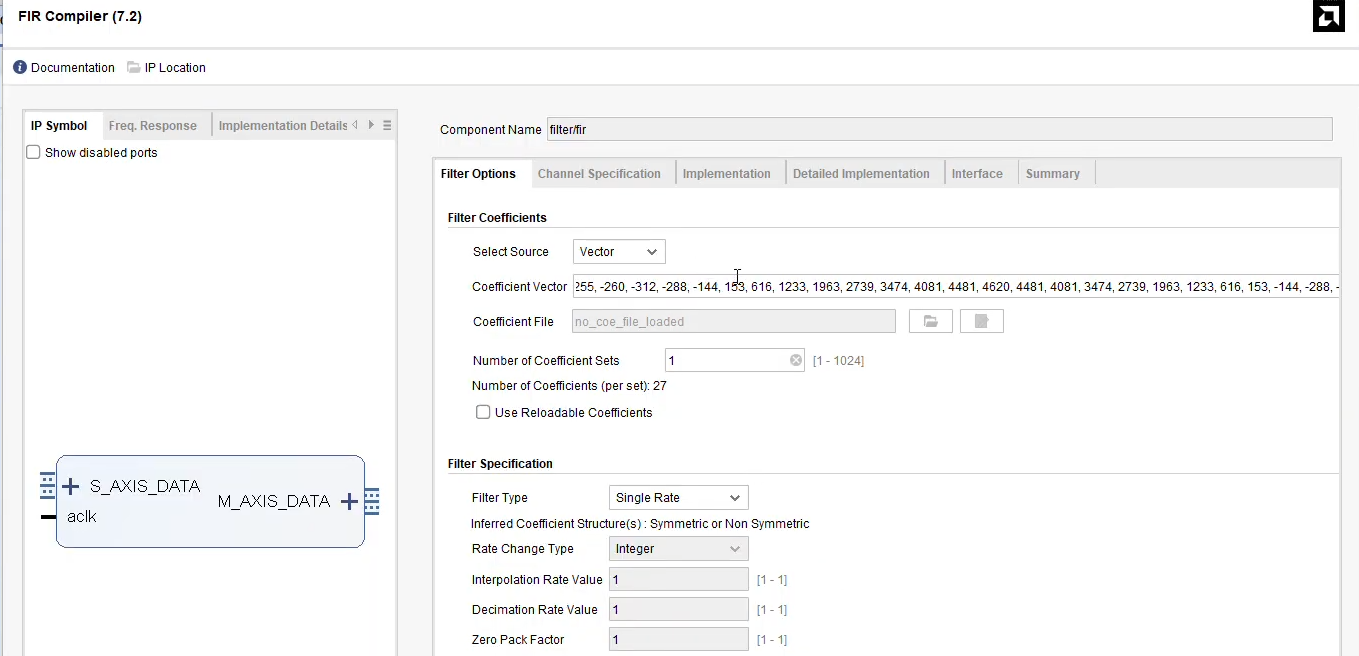
\includegraphics[width=0.47\textwidth]{Coeff_config.png}}
		\caption{Coefficient configuration and filter settings in Vivado FIR Compiler.}
		\label{fig_coeff}
	\end{figure}
	
	\subsection{Hierarchy Overview}
	Fig.~\ref{fig_hier} illustrates the filter hierarchy within the Vivado design, which includes both the FIR Compiler and the DMA interfaces that facilitate data transfer between the PS and PL.
	
	\begin{figure}[htbp]
		\centerline{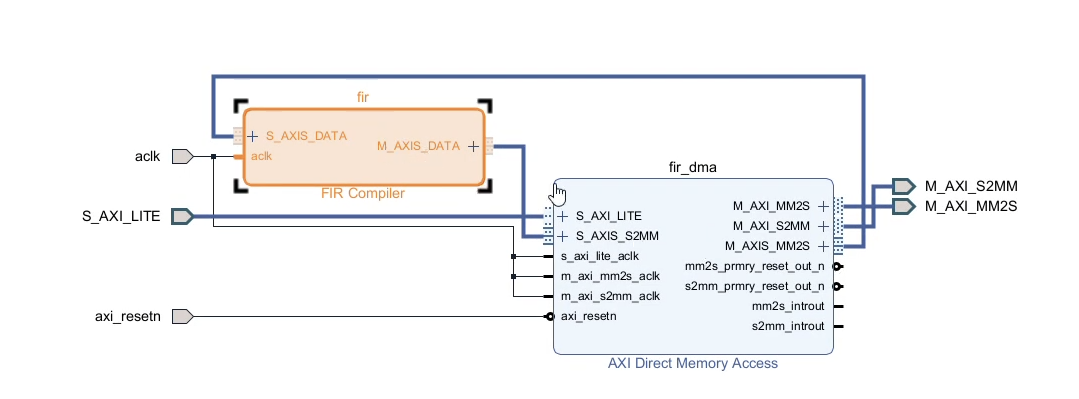
\includegraphics[width=0.47\textwidth]{Heirarchy.png}}
		\caption{Vivado project hierarchy showing FIR Compiler and DMA connectivity.}
		\label{fig_hier}
	\end{figure}
	
	\subsection{Complete System Block Diagram}
	The full Zynq system configuration connecting the PS, DMA, and FIR Compiler IPs is shown in Fig.~\ref{fig_fullblock}.
	
	\begin{figure}[htbp]
		\centerline{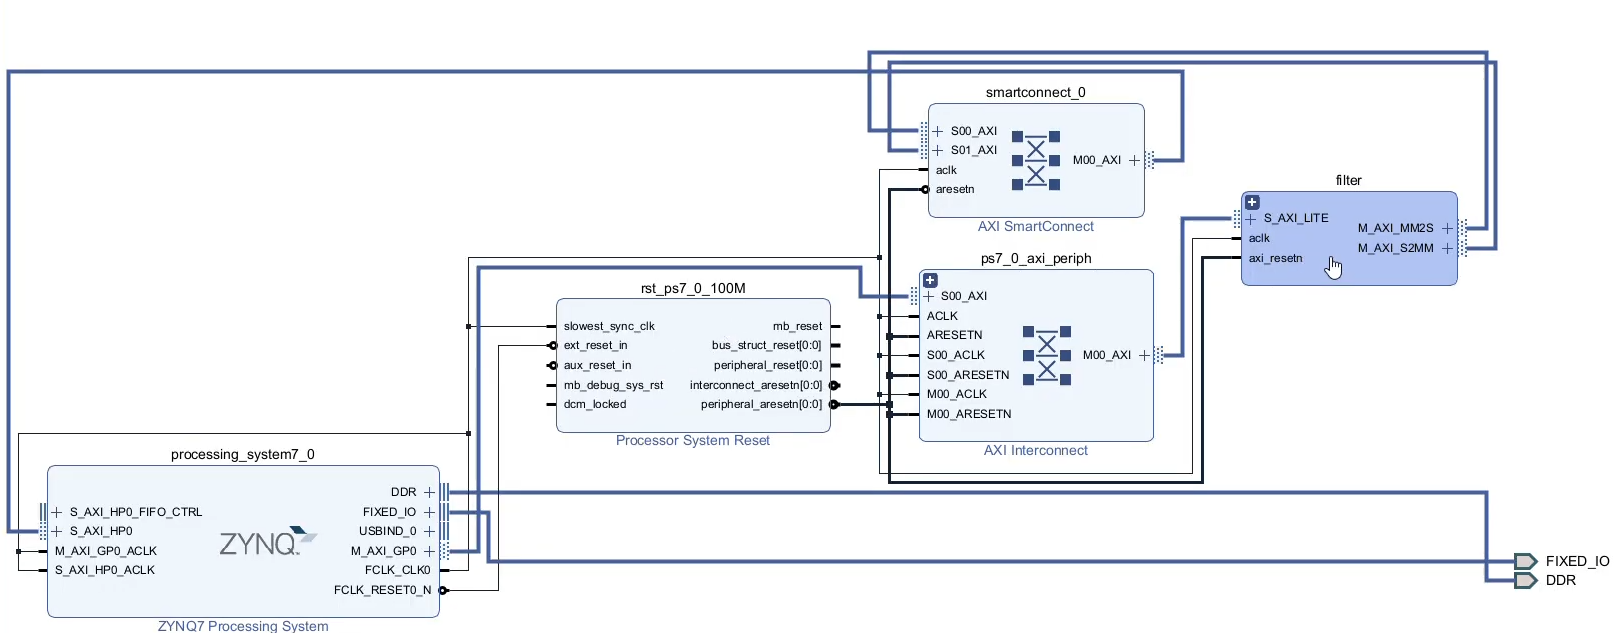
\includegraphics[width=0.47\textwidth]{complete_block_diagram.png}}
		\caption{Complete block diagram of Zynq-FIR system with DMA interfacing.}
		\label{fig_fullblock}
	\end{figure}
	
	\section{Implementation and Resource Utilization}
	The synthesis and implementation were performed using Xilinx Vivado. The FIR Compiler-based implementation consumed the following hardware resources:
	
	\begin{table}[htbp]
		\caption{Resource Utilization Summary}
		\begin{center}
			\begin{tabular}{|l|c|}
				\hline
				\textbf{Resource} & \textbf{Usage} \\
				\hline
				LUTs & 5244 \\
				Slice Registers & 7307 \\
				Block RAMs & 2 \\
				DSP Slices & 29 \\
				IO Ports & 130 \\
				BUFGCTRL & 1 \\
				\hline
			\end{tabular}
			\label{tab_resources}
		\end{center}
	\end{table}
	
	For comparison, a standard HLS-based implementation (without using the FIR Compiler IP) required 7017 LUTs, 12106 FFs, 4 BRAMs, and 297 DSP slices with a latency of 233 cycles ($2.33 \times 10^3$ ns). Given that the PYNQ Z2 board supports only 220 DSP slices, the FIR Compiler design proved more resource-efficient and feasible.
	
	\section{Results and Discussion}
	Simulation results verified the functional correctness of the FIR filter. Fig.~\ref{fig_result1} shows the input distorted sine wave and the reconstructed (filtered) sine wave, confirming proper filtering behavior.
	
	\begin{figure}[htbp]
		\centerline{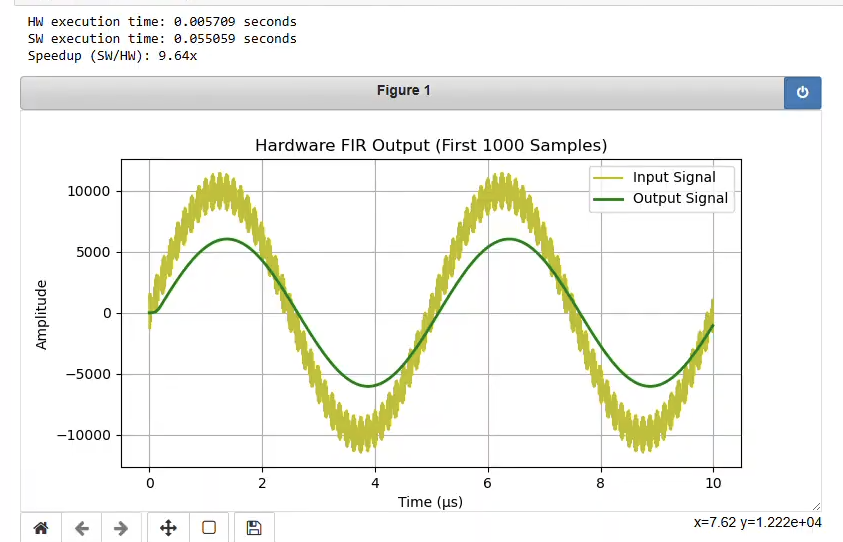
\includegraphics[width=0.47\textwidth]{result1.png}}
		\caption{Input distorted sine wave and output reconstructed sine wave.}
		\label{fig_result1}
	\end{figure}
	
	The hardware (PL) execution time was measured at 0.005709 seconds, while the software (PS) execution required 0.055059 seconds, as summarized in Fig.~\ref{fig_result2}. This demonstrates a nearly 10$\times$ performance gain using hardware acceleration.
	
	\begin{figure}[htbp]
		\centerline{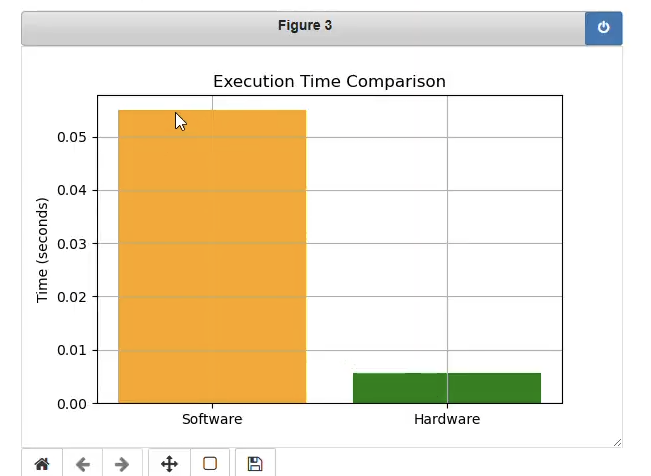
\includegraphics[width=0.47\textwidth]{result2.png}}
		\caption{Comparison of hardware and software execution times.}
		\label{fig_result2}
	\end{figure}
	
	\section{Conclusion}
	The implementation of an FIR filter using the Vivado FIR Compiler IP on a Zynq SoC demonstrated substantial improvements in both performance and resource efficiency. The integration of the FIR Compiler with DMA and PS-PL communication enables high-throughput real-time filtering. Future work involves implementing adaptive FIR filters and exploring higher tap counts with optimized resource sharing.
	
	\section*{Acknowledgment}
	The author would like to thank the faculty mentors and hardware team at RMK Engineering College for their support in realizing the FPGA implementation.
	
	\begin{thebibliography}{00}
		\bibitem{b1} Xilinx Inc., ``Vivado Design Suite User Guide: FIR Compiler (UG073),'' 2022.
		\bibitem{b2} Zynq-7000 SoC Technical Reference Manual, Xilinx, 2021.
		\bibitem{b3} A. K. Jain, ``Digital Signal Processing: Principles, Algorithms, and Applications,'' Pearson, 2019.
		\bibitem{b4} Kartik Agrawal, Abhijit Asati, ``Improved Implementation of PYNQ-Based FFT Hardware Accelerator,'' IEEE, 2024.
		\bibitem{b5} A.E. Cetin, O.N. Gerek, Y. Yardimci, ``Equiripple FIR Filter Design by the FFT Algorithm,'' IEEE, 2024.
		\bibitem{b6} Guoyong Wang, ``Implementation of FIR Digital Filter Algorithm in C Language on DSP Platform,'' IEEE, 2024.
		\bibitem{b7} Xiao Liangfen, Liu Yi, ``Implementation of Distributed FIR Digital Filter on FPGA,'' IEEE, 2023.
	\end{thebibliography}
	
	\vspace{12pt}
	
\end{document}
